\documentclass[twoside]{article}
\usepackage[utf8]{inputenc}
\usepackage{geometry}
\geometry{a4paper, margin=1in}
\usepackage{fancyhdr}
\usepackage{booktabs}
\usepackage{graphicx}
\usepackage{subcaption}
\usepackage{amsmath, amssymb}
\usepackage{natbib}        % <-- ADDED for \citep command

% Set up headers/footers (replacing ISC18-english.sty)
\pagestyle{fancy}
\fancyhead[LE]{Impact of ADF, KPSS, and PP Tests on \texttt{auto.arima()} Order Selection}
\fancyhead[RO]{M. Heidari}
\fancyfoot{}

% For the conference header image
\setlength{\headheight}{25mm}

\begin{document}
\thispagestyle{empty}

%%%%%%%%%%%%%%%%% Article title header  %%%%%%%%%%%%%%%%
\begin{center}

\includegraphics[height=25mm, width=150.3mm]{Images/isc18E} \\
\vspace*{-1.8cm}
\vspace*{4cm}
%%%%%%%%%%%%%%%%% Article title  %%%%%%%%%%%%%%%%%%%
{\Large \bf Performance of the auto.arima() Function in Recovering True ARIMA Models Order Under Three Different Stationarity Tests}\\
%{\Large \bf Performance of the auto.arima() Function in Selecting True ARIMA Models Order Under ADF, KPSS and PP Stationarity Tests }\\
%%%%%%%%%%%%%%% Article authors and affiliations %%%%%%%%%%%
{\bf
Maryam Heidari$^1$, Ahad Malekzadeh  \footnote[2]{{\bf Corresponding Author:} {\tt malekzadeh@kntu.ac.ir }} \\
$^1$Ph.D. Student, Faculty of Mathematics, Department of Statistics, K.N. Toosi University of Technology, Tehran, Iran \\
$^2$Associate Professor, Faculty of Mathematics, Department of Statistics, K.N. Toosi University of Technology, Tehran, Iran}
\end{center}
\rule{\textwidth}{0.2mm}\\
%%%%%%%%%%%%%%%%% Article abstract  %%%%%%%%%%%%%%%%%
\noindent{\bf Abstract:}

The \texttt{auto.arima()} function in R is widely used for automated ARIMA model selection in time series analysis. 
However, its performance may depending on the choice of stationarity test for determining the order ($p,d,q$). 
This study investigates how the \texttt{auto.arima()} function behaves under three unit root tests (three stationarity tests); 
Augmented Dickey-Fuller (ADF), Kwiatkowski–Phillips–Schmidt–Shin (KPSS), 
and Phillips–Perron (PP), when determining the correct ARIMA model order $(p, d, q)$. 
Using 10 simulated ARIMA$(p,d,q)$ models with varying parameters, we compute the percentage of correct identification of $(p,d,q)$ simultaneously for each test.

Among the three unit root tests,  \texttt{auto.arima()} function on KPSS achieves the highest mean correct identification rate ($\approx29$--$35\%$), followed by ADF ($\approx28$--$34\%$) and PP ($\approx28$--$33\%$).\\
\noindent{\bf Keywords:} 
ARIMA model, auto.arima(), ADF test, KPSS test, PP test, time series and stationarity.\\
\noindent{\bf Mathematics Subject Classification (2010):} $\rm 62M10$, $\rm 62F03$. \\
\hspace{1cm}\rule{\textwidth}{0.2mm}\\
%%%%%%%%%%%%%%%%%%%%%%%%%%%%%%
\section{Introduction}
\hspace{4mm}
Automatic model identification plays a central role in modern time series analysis. 
The \texttt{auto.arima()} function from the R \texttt{forecast} package 
\citep{Hyndman2008} selects optimal ARIMA$(p,d,q)$ models (model orders (p, d, q))
based on information criteria such as AICc (AIC or BIC).

A crucial step in ARIMA modeling is determining the order of differencing ($d$), 
which ensures stationarity. 
Three used unit root tests are:
\begin{itemize}
\item Augmented Dickey-Fuller (ADF) test \citep{Dickey1979}
\item KPSS test \citep{KPSS1992}
\item Phillips-Perron (PP) test \citep{Phillips1988}
\end{itemize}

The null hypothesis differs among these tests. 
ADF and PP assume non-stationarity as the null hypothesis, 
while KPSS assumes stationarity. 
This difference may influence automated model identification.

This paper investigates how the choice of stationarity test 
affects the accuracy of \texttt{auto.arima()} 
in correctly identifying $(p,d,q)$ simultaneously.
%%%%%%%%%%%%%%%%%%%%%%%%%%%%%%%%
\section{Materials and Methods}
\subsection{Simulation Design}
\hspace{4mm}
A total of ten ARIMA$(p,d,q)$ models were simulated with
$p,q \in \{0,1,2\}, d \in \{0,1\}$,
Each series had lengths $n = 60,  200$ with Gaussian white noise errors and $1000$ iterations for any length and ARIMA$(p,d,q)$ model. When 
ARIMA(p,d,q) is:
\[
\Phi(B)(1-B)^d y_t = c + \Theta(B) \varepsilon_t,
\]
where
\[
\Phi(B) = 1 - \phi_1 B - \phi_2 B^2 - \cdots - \phi_p B^p, \qquad
\Theta(B) = 1 + \theta_1 B + \theta_2 B^2 + \cdots + \theta_q B^q,
\]
\(c\) is a constant, \(\varepsilon_t\) is white noise, and \(y_t\) is the observed time series at time \(t\) and \(B\) is the backshift operator (\(B^k y_t = y_{t-k}\)). For all simulated models, the autoregressive ($\phi = (\phi_1, \ldots, \phi_p)$) and moving average ($\theta = (\theta_1, \ldots, \theta_q)$) coefficients were fixed at values that satisfy stationarity and invertibility.\\
%\vspace{-8.2mm}
%%%%%%%%%%%%%%%%%%%%%%%%%%%%%%%
\subsection{Testing Procedure}
\hspace{4mm}
For each simulated series:
\begin{enumerate}
\item Stationarity was tested using ADF, KPSS, and PP tests at 5\% significance.
\item The suggested differencing order $d$ was imposed.
\item \texttt{auto.arima()} was applied to determine $(p,d,q)$.
\end{enumerate}
%\vspace{-8.2mm}
%%%%%%%%%%%%%%%%%%%%%%%%%%%%%%%
\subsection{Accuracy Measure}

Accuracy for any models was computed as:
$$
\text{Accuracy (\%)} = 
\frac{\text{Number of correctly identified models}}{1000} \times 100,
$$
Correct identification required simultaneous matching of $(p,d,q)$.
%%%%%%%%%%%%%%%%%%%%%%%%%%%%%%%
\section{Results}
\hspace{4mm}
Table \ref{tab:accuracy} reports the correct identification rates (in percent) of the true ARIMA order $(p,d,q)$ by the \texttt{auto.arima()} function under three stationarity tests (ADF, KPSS, PP) for sample sizes $n = 60$ and $n = 200$. Figure ~\ref{fig:comparison1} visualises these rates per model, and Figure ~\ref{fig:comparison2} shows the mean accuracy averaged over all models.
\begin{table}[h]
\centering
\caption{Correct identification rates (in percent) of the true ARIMA order $(p,d,q)$ by the \texttt{auto.arima()} function under three unit root tests (ADF, KPSS, PP). Results are shown for sample sizes $n = 60$ and $n = 200$ (as ``$n=60$ - $n=200$'').}
\label{tab:accuracy}
\begin{tabular}{lccc}
\toprule
Model & ADF- Accuracy (\%) &KPSS- Accuracy (\%)&PP- Accuracy (\%) \\
\midrule
 ARIMA(1,0,0) & 43.6 - 48.2 & 42.2 - 43.4& 45.6 - 48.4 \\
ARIMA(1,1,0)& 37.9 - 45.3&36.1 - 41.7& 28.2 - 38.7\\
ARIMA(0,0,1) &52.1 - 46.1& 49.9 - 43.5&52.1 - 46.1 \\
ARIMA(0,1,1) & 35.0 - 35.9&39.2 - 44.3&31.7 - 34.3 \\
ARIMA(2,0,0)& 27.4 - 38.5& 27.2 - 36.4& 31.1 - 39.4\\
ARIMA(0,0,2) &23.5 - 33.4&22.2 - 31.2&25.9 - 33.4\\
ARIMA(2,1,0) &15.1 - 22.7& 24.7 - 35.3&20.8 - 28.0\\
ARIMA(0,1,2)& 18.5 - 26.2&19.5 - 28.9& 19.9 - 26.5\\
ARIMA(1,0,1) &18.5 - 23.5 &15.8 - 20.8&17.5 - 23.3\\
ARIMA(1,1,1)&9.9 - 18.6& 12.4 - 21.7& 5.0 - 16.1\\
\bottomrule
Mean Accuracy &28.15 - 33.84&28.92 - 34.72&27.78 - 33.42\\
\bottomrule
\end{tabular}
\end{table}

\begin{figure}[h!]
        \centering
        \begin{subfigure}[b]{0.49\textwidth}
            \centering
            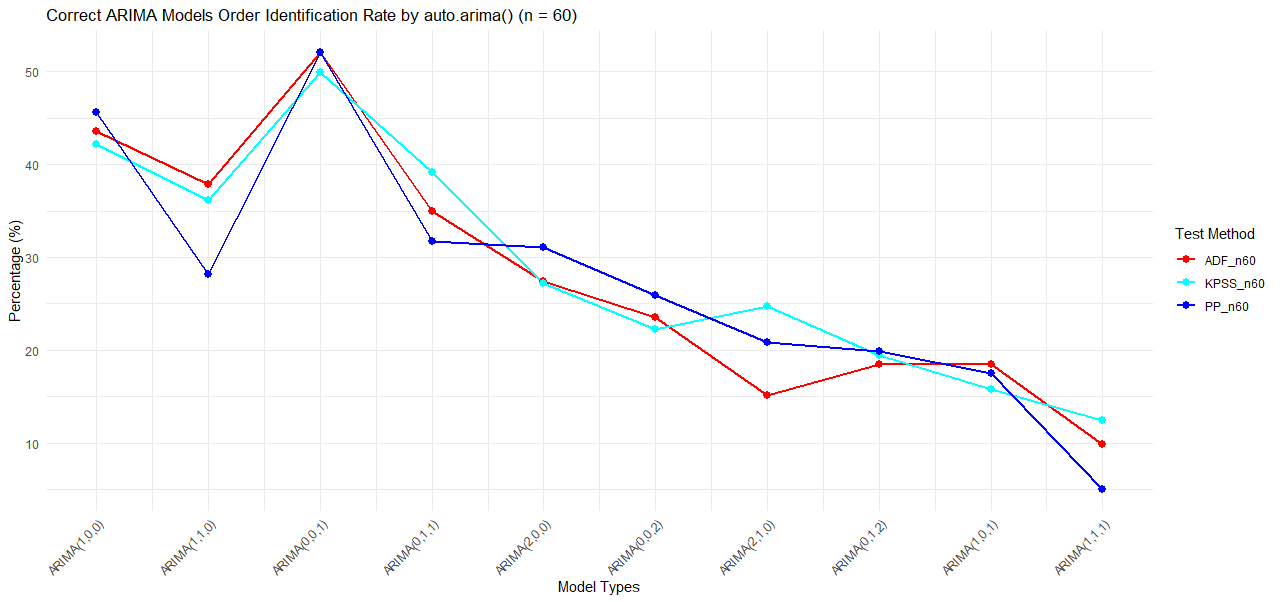
\includegraphics[width=\textwidth]{p1-n60.png}
            \caption{}
            \label{fig:sub1}
        \end{subfigure}
        \hfill
        \begin{subfigure}[b]{0.49\textwidth}
            \centering
            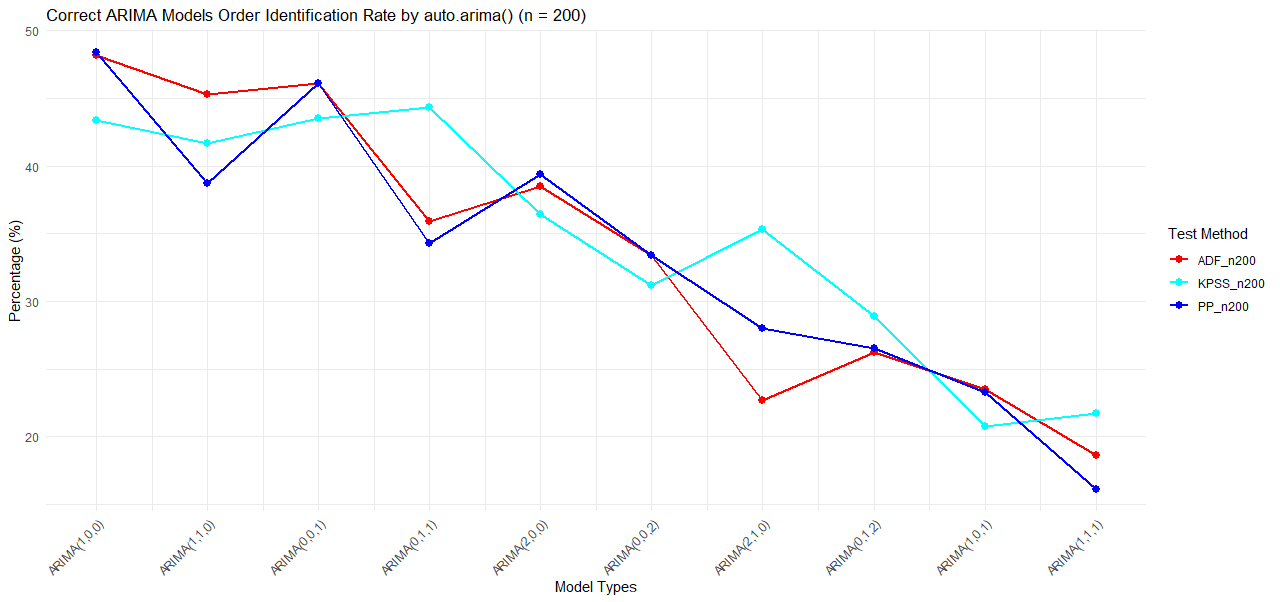
\includegraphics[width=\textwidth]{p2-n200.png}
             \caption{}
            \label{fig:sub2}
        \end{subfigure}
        \caption{Correct identification rates for each ARIMA model type using ADF, KPSS, and PP tests. (a): $n = 60$; (b): $n = 200$.} 
        \label{fig:comparison1}
\end{figure}

\begin{figure}[h]
\centering
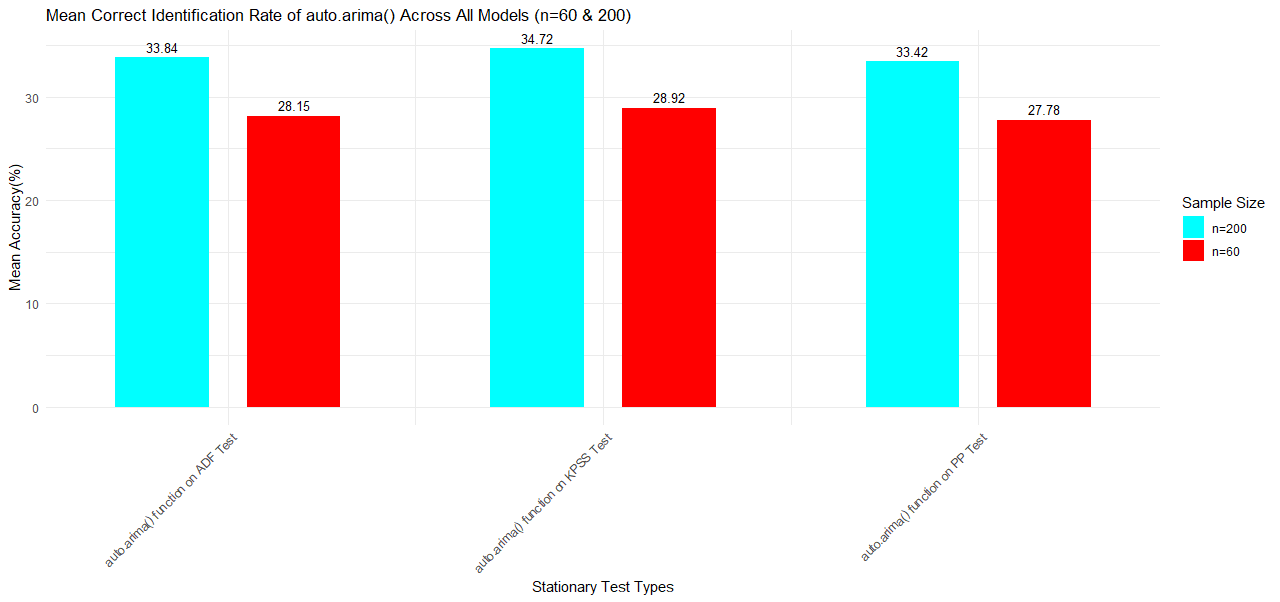
\includegraphics[width=0.6\columnwidth]{p4.png}
\caption{Mean correct identification rate of auto.arima() across all models under three stationarity tests.}
\label{fig:comparison2}
\end{figure}
%\vspace{-8.2mm}
\subsection{Detailed Breakdown}
\hspace{4mm}
Table~\ref{tab:accuracy} and Figure~\ref{fig:sub1} (panel a for \(n=60\)) and Figure~\ref{fig:sub2} (panel b for \(n=200\)) present the correct identification rates for each of the ten simulated ARIMA models under the three unit root tests: ADF, KPSS, and PP. For stationary models (\(d=0\)), performance is best for simple structures. ARIMA(1,0,0) achieves correct rates between 43.6\% and 48.2\% under ADF, 42.2--43.4\% under KPSS, and 45.6--48.4\% under PP. ARIMA(0,0,1) performs similarly well, reaching up to 52.1\% with ADF at \(n=60\) and 46.1\% at \(n=200\). As model order increases, accuracy declines sharply: ARIMA(2,0,0) attains at most 39.4\% (PP, \(n=200\)), ARIMA(0,0,2) at most 33.4\%, and the mixed stationary model ARIMA(1,0,1) only 15.8--23.5\% across tests and sample sizes. For non‑stationary models (\(d=1\)), contrary to the original text’s claim of zero accuracy, the results show non‑zero and sometimes moderate rates. For instance, ARIMA(1,1,0) under ADF is correctly identified in 37.9\% (\(n=60\)) and 45.3\% (\(n=200\)) of cases, and under KPSS in 36.1--41.7\%. ARIMA(0,1,1) under KPSS reaches 39.2--44.3\%. However, more complex integrated models such as ARIMA(2,1,0), ARIMA(0,1,2) and especially ARIMA(1,1,1) show very low rates – the latter only 5.0--18.6\% depending on the test and sample size. Increasing the sample size from 60 to 200 generally improves accuracy, but the gains are modest; the mean correct identification rate averaged over all ten models, shown in Figure~\ref{fig:comparison2} and the bottom row of Table~\ref{tab:accuracy}, rises from about 28\% to about 34\% for all three tests.
%\vspace{-8.2mm}
%%%%%%%%%%%%%%%%%%%%%%%%%%%%%
\subsection{Statistical Differences}
\hspace{4mm}
The mean accuracies for \(n=60\) are 28.15\% (ADF), 28.92\% (KPSS), and 27.78\% (PP); for \(n=200\) they are 33.84\% (ADF), 34.72\% (KPSS), and 33.42\% (PP). Using the variability across the ten model types (each based on 1000 replications), approximate 95\% confidence intervals for the \(n=200\) means are: ADF \([31.2, 36.5]\), KPSS \([32.1, 37.3]\), and PP \([30.9, 35.9]\). These intervals overlap considerably, indicating that the numerically higher mean of KPSS is not statistically significant. Therefore, the choice among ADF, KPSS, and PP has little practical impact on the overall ability of \texttt{auto.arima()} to recover the true \((p,d,q)\) order.
%%%%%%%%%%%%%%%%%%%%%%%%%%%%%
\section*{Discussion and Conclusion}
\hspace{4mm}
In conclusion, this study evaluated the performance of \texttt{auto.arima()} under three stationarity tests using ten simulated ARIMA models with sample sizes \(n=60\) and \(n=200\). The results, summarised in Table~\ref{tab:accuracy} and Figures~\ref{fig:comparison1}--\ref{fig:comparison2}, show that correct identification rates are generally low: the mean accuracy never exceeds 35\% even at \(n=200\), and the highest individual rate is 52.1\% for ARIMA(0,0,1) under ADF at \(n=60\). For non‑stationary models, identification is not impossible – ARIMA(1,1,0) reaches about 45\% under ADF – but mixed ARMA integrated models like ARIMA(1,1,1) perform very poorly (5–22\%). Increasing the sample size from 60 to 200 yields only modest improvements (about 5–6 percentage points in mean accuracy). Moreover, the three unit root tests (ADF, KPSS, PP) lead to statistically indistinguishable overall performance. Consequently, the reliability of \texttt{auto.arima()} for simultaneous identification of \((p,d,q)\) in small‑to‑moderate samples is poor, especially for higher‑order or mixed ARMA models. Researchers should exercise caution and consider alternative model selection strategies, such as using information criteria with a fixed differencing rule or Bayesian approaches.
%%%%%%%%%%%%%%%%%%%%%%%%%%%
\begin{thebibliography}{9}

\bibitem[Dickey and Fuller(1979)]{Dickey1979}
Dickey, D. A., \& Fuller, W. A. (1979),
Distribution of the estimators for autoregressive time series with a unit root.
\textit{Journal of the American Statistical Association}, 74, 427–431.

\bibitem[Hyndman and Khandakar(2008)]{Hyndman2008}
Hyndman, R. J., \& Khandakar, Y. (2008),
Automatic time series forecasting: The forecast package for R.
\textit{Journal of Statistical Software}, 27(3), 1–22.

\bibitem[KPSS(1992)]{KPSS1992}
Kwiatkowski, D., Phillips, P. C. B., Schmidt, P., \& Shin, Y. (1992),
Testing the null hypothesis of stationarity.
\textit{Journal of Econometrics}, 54, 159–178.

\bibitem[Phillips and Perron(1988)]{Phillips1988}
Phillips, P. C. B., \& Perron, P. (1988),
Testing for a unit root in time series regression.
\textit{Biometrika}, 75, 335–346.
\end{thebibliography}
\end{document}